%!TEX root = ../thesis

\chapter{Simulation} % (fold)
\label{cha:simulation}

\section{Model and Simulation Protocol} % (fold)
\label{sec:model_and_simulation_protocol}

The simulation protocol was mostly carried over from \cite{wettermann_minimal_2020}. The main file for simulating the genome structure of an entire cell is \verb|simulate_cell.py|; additionally simulations of single chromosomes were carried out, the protocol for these simulations is identical to that of the entire genome, except only the beads of the chromosome in question were modelled. The simulation is a molecular dynamics simulation using the HOOMD-blue\cite{anderson_hoomd-blue_2020} toolkit. It utilises a Langevin integrator (\verb|hoomd.md.integrate.langevin| with a timestep of \(dt=0.001\), a temperature of \(kT = 1.0\)), and a drag coefficient of \(\gamma = 1.0\). The neighbor list is a BVH tree neighbour list \cite{howard_efficient_2016} \cite{howard_quantized_2019} that was originally chosen as it scales
with particle number as opposed to the system volume\cite{wettermann_minimal_2020}.

Each chromosome is modelled as beads on a string, where each bead represents a bin of \(\SI{100000}{bp}\). This is the same resolution as was chosen in \cite{wettermann_minimal_2020}, and represents a compromise between the resolution of our simulation and the \textcolor{orange}{resolution}\todo{find better word} of the contact data we have available: a higher resolution, i.e. a smaller bin size of for example \(\SI{40000}{bp}\), would increase the resolution of our simulation and enable us to see smaller structures, but at the same time would spread our fixed number of contacts across a higher number of beads. This would make in particular the effect of having captured only a fraction of all possible contacts in the cell using Hi-C more prominent.\todo{insert reference to table of fraction of contacts captured} Vice versa, decreasing the bin size would help mitigate the partial capture of contacts, but limit our spatial resolution in the simulation. With this resolution our genome is represented by 20 chains varying in length between 500 and 2,000 beads (the exact lengths for each chromosome can be found in Table~\ref{tab:chrom_lengths}), or 25,714 beads in total. This does not represent the entirety of the mouse genome, whose length is approximately \(\SI{2632}{Mbp}\)\footnote{Mouse Genome Assembly GRCm39 from \url{https://www.ncbi.nlm.nih.gov/grc/mouse/data}, visited on 26.02.2022}, or 26,321 beads at our resolution of \(\SI{100000}{bp \per bead}\). The reason for this is that beads at the boundary of a chromosome that had no contact in any of the eight cells were dropped from the simulation, since their impact was assumed to be only very small. Boundary beads that had contacts in some cells but not others were kept in the simulation of all cells in order to keep the simulation data comparable across cells.

The model is based on a generic bead-spring polymer model in which three kinds of bonds are defined. The first two kind of bonds are harmonic bonds between two beads with the general protential

\[
  V(r) = \frac{2} \kappa \left( r - r_0 \right)^2
\]

where \(\kappa\) is the force constant determining the stiffness of the bond, which is set at \(\kappa = 2000\) for all harmonic bonds, and \(r_0\) is the preferred bond distance. The first kind of harmonic bonds are the backbone bonds connecting adjacent beads in each chromosome. For these bonds the preferred distance is set to \(r_0 = 1.0 \). The other harmonic bonds in the simulation are the pre-defined contacts derived from the Hi-C data set from\cite{stevens_3d_2017}. Here the preferred bond distance is set a little bit larger compared to the backbone at \(r_0 = 1.5\) in accordance with \cite{wettermann_minimal_2020}.

The third kind of bond is a Gaussian pair potential of the form

\[
  V(r) = \begin{cases}
    \epsilon \exp \left[ - \frac{2} \left( \frac{r}{\sigma} \right)^2 \right] & r < r_\text{cut} \\
    0 & r \geq r_\text{cut}
  \end{cases}
\]

between all beads designed to push all non-bonded beads away from each other. This potential is used in 2 forms in different parts of the simulation: a full form with \(\sigma = 1.0\) and \(r_\text{cut} = 3.5\) and a reduced form with \(\sigma = 0.1\) and \(r_\text{cut} = 0.4\). In both cases \(\epsilon = 100\). On one hand, this reproduced the fact that at physiological conditions DNA is negatively charged and thus repels each other. \textcolor{orange}{On the other hand it represents an excluded volume potential that pushes all beads away from each other}\todo{Rewrite?}. An overview of all the potentials in the simulation can be seen in Figure~\ref{fig:potentials}.

\begin{figure}[ht]
\centering
  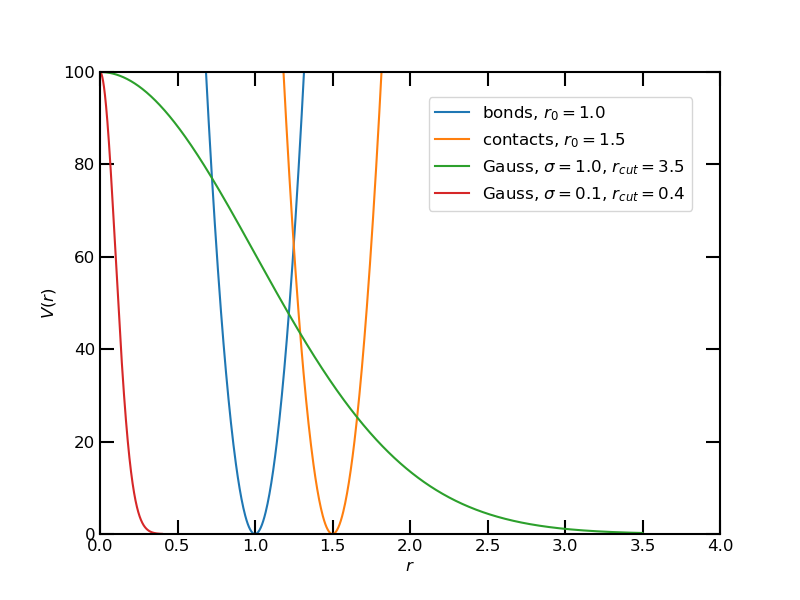
\includegraphics[width=\figwidth]{potentials.png}
  \caption{Potentials used in the simulation. Bonds and contacts are harmonic potentials of the form \(V(r) = 1000 (r - r_0)^2\), with bonds having an \(r_0\) of 1.0 and contacts gaving an \(r_0\) of 1.5. Gauss potentials are of the form \(V(r) = 100 \exp\left[- \frac{2} \left( \frac{r}{\sigma} \right)^2 \right]\) and are set to 0 for \(r\) greater than the cutoff value \(r_\text{cut}\).}
  \label{fig:potentials}
\end{figure}

The system is initalised by distributing all the beads randomly throughout the simulation box (uniform distribution, using \verb|numpy.uniform.random|\cite{harris_array_2020}). The bonds are set and the simulation is repeatedly run \textcolor{orange}{through} the following steps:

\begin{itemize}[label=\(\bullet\)]
  \item 80,000 time steps with no excluded volume potentials
  \item 50,000 time steps with reduced volume potentials
  \item 50,000 time steps with full excluded volume potentials
\end{itemize}

Bonds and contacts are active at all of those steps. After each cycle the current state is saved to a gsd trajectory file. These states will be referred to in the following as a \textbf{frame}. Frames whose trajectory are similar are said to belong to the same \textbf{configuration}.\todo{Definition of term here?} These steps were repeated in each simulation for a total of 105 cycles. The first few cycles have to be discarded as the system takes some time to find its ground state, although certain problems can arise here that will be discussed later in \ref{sec:problems_with_the_simulation}.

% section model_and_simulation_protocol (end)

\section{Simulation results} % (fold)
\label{sec:simulation_results}

Each simulation will yield 105 sequential configuration, i.e. the simulation state is not reset after each simulation cycle, but instead the final state of each cycle is the initial state of the next cycle. This has the advantage of giving the system time to \textcolor{orange}{tune in}\todo{better word? \enquote{einschwingen}}, but also the disadvantage of the possiblility that certain end configurations will never be reached in a simulation run after it has tuned in to a different locally minimal configuration. The potential energies of the simulation run of cell 2 can be seen in Figure~\ref{fig:potential_energy_cell2}. The first two configurations show a potential energy significantly larger than the later ones, then the system quickly converges to a potential energy of about \(\num{7950000}\) and shows only small deviations of less than \(1 \%\). Thus both the length of the settling period and the potential energy of the configurations match \cite{wettermann_minimal_2020} extremely well. \textcolor{orange}{To minimise the effect of the settling period the first 5 configurations of each simulation run will generally be excluded in all subsequent analyses where the data from all configurations are combined.}

Likewise, Figure~\ref{fig:distance_pdf_cell2} shows the distance distribution of the bonds and (predetermined) contacts across all configurations of the simulation of cell 2. The results are again very similar to \cite{wettermann_minimal_2020}, with both peaks and means shifted slightly to the right. The \(99.73\)th quartile is at \(1.713\) for bonds and \(2.418\) for contacts, showing that most bonds and contacts are enforced reasonably well.

\begin{figure}[ht]
\centering
  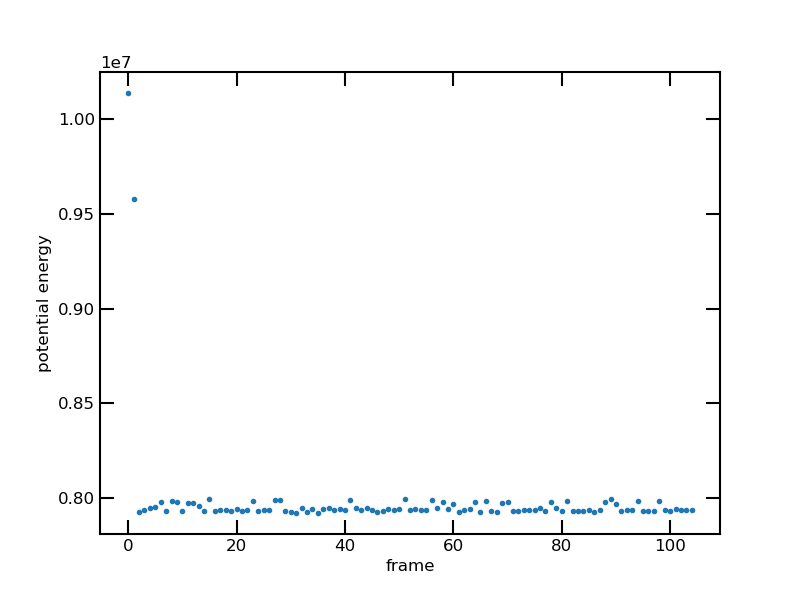
\includegraphics[width=12cm]{potential_energy_cell2.png}
  \caption{\textcolor{red}{CAPTION}}
  \label{fig:potential_energy_cell2}
\end{figure}

\begin{figure}[ht]
\centering
  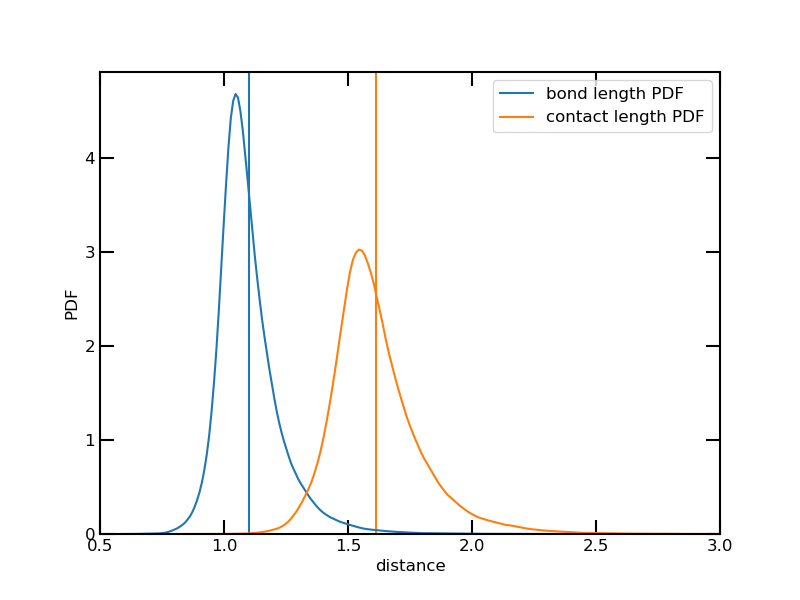
\includegraphics[width=12cm]{distance_pdf_cell2.png}
  \caption{\textcolor{red}{CAPTION} bond mean: \(\num{1.099}\) ; bonds \(99.73\%\) percentile: \(1.713\) ; contacts mean: \(\num{1.613}\) ; contact \(99.73\%\) percentile: \(2.418\)}
  \label{fig:distance_pdf_cell2}
\end{figure}

For the other cells the situation is generally similar, except for cell 1 and cell 5, which will be dicussed separately in \ref{sec:problems_with_the_simulation}. The standard deviations of potential energies are between \(0.3\%\) and \(1.8\%\) of the mean, showing the minimum energy configuration to be quite stable in these cells. Also neither bonds nor contacts are overly overstretched in any cells, including cell 1 and cell 5. A complete overview of potential energy percentage standard deviations and mean and \(99.73\)th percentile for bonds and contacts can be found in Table~\ref{tab:simulation_pe_dists}.

Renderings of all simulated cells can be seen in Appendix~\ref{cha:renderings_of_simuated_cells}. A few things can be notes from these images visually.

First, most simulated genomes have a quite regular, spherical shape, but in particular cell 3, cell 8, and the higher energy configuration of cell 5 (which will be discussed in more detail in \ref{sec:problems_with_the_simulation}) show clear differences from this. Cell 3 and cell 8 have a more elongated, bean-like shape, as can be seen in Figure~\ref{img:cell3_frame104_scene1} for cell 3 and in Figure~\ref{img:cell8_frame104_scene2} for cell 8. The higher energy configuration of cell 5 on the other hand has a more obloid, donut-like shape. Another notable \textcolor{orange}{thing} is that cell 6 and cell 7 are hollow as can be seen for example in Figure~\ref{img:cell6_frame104_scene1} for cell 6 and Firgure~\ref{img:cell7_frame104_scene1} for cell 7.

% section simulation_results (end)

\section{Problems with the simulation} % (fold)
\label{sec:problems_with_the_simulation}

There were certain problems arising with the simulation itself.

\subsection{Cell 1} % (fold)
\label{sub:cell_1}

\textcolor{orange}{In cell 1, a ground state was reached very quickly, but this ground state is very unstable, as shown in Figure~\ref{fig:potential_energy_cell1}.} The RMSDs of all frames with respect to the last frame, which is of ground state energy, seen in Figure~\ref{fig:rmsd_cell1} shows that some of these frames have rather similar configurations while others are very different. The obvious hypothesis would be to assume that it is the low energy frames that are similar to each other and the high energy frames that are more different. This can be tested by selecting all frames with low energy, defined by being below some cutoff energy, and checking how the RMSDs for those frames behaves. A cutoff energy of \(\num{1.495e7}\), visually displayed in Figure~\ref{fig:potential_energy_cell1} as the orange line, was chosen as it captures most of the frames that can be identified in Figure~\ref{fig:potential_energy_cell1} as being low energy, while excluding all that deviate strongly from this baseline energy. This selects a total of 52 frames, which have been marked in Figure~\ref{fig:rmsd_cell1} by red dot. As can be seen very clearly, these low energy frames do in fact have a very low RMSD of \(\num{1.00(1)}\) with respect to the last frame. This confirms that while it is very unstable, this simulation of cell 1 does in fact have a ground state, and we can filter it out of all frames by selecting for those with a low energy. To check if this ground state instability is an intrinsic property of the setup for cell 1 or merely a random artifact of the simulation, cell 1 was simulated two more times. The potential energies for those repeated simulations can be seen in Figure~\ref{fig:potential_energy_cell1_1} and Figure~\ref{fig:potential_energy_cell1_2} in the appendix and clearly show the same pattern of instability, leading to the conclusion that this instability is in fact a consequence of the predetermined contacts for cell 1.

\begin{figure}[ht]
\centering
  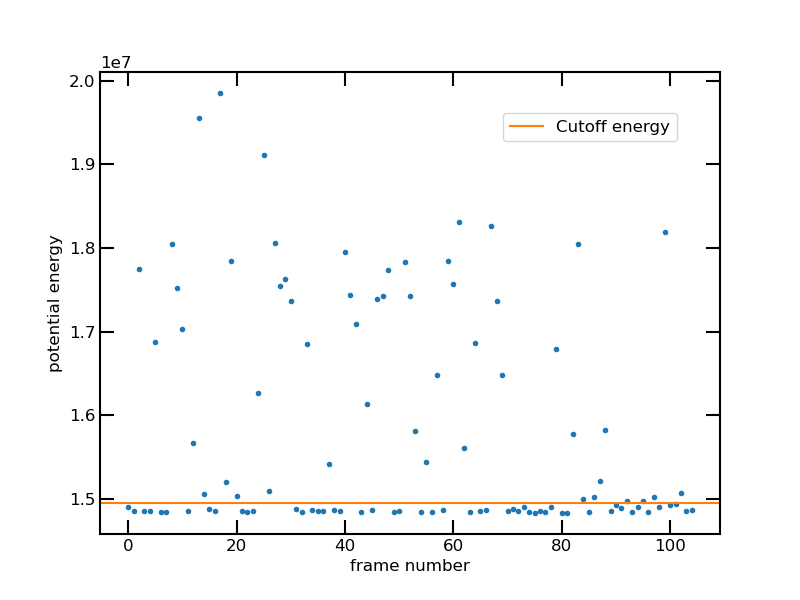
\includegraphics[width=\figwidth]{potential_energy_cell1.png}
  \caption{Potential energies of the frames in the simulation of cell 1.}
  \label{fig:potential_energy_cell1}
\end{figure}

\begin{figure}[ht]
\centering
  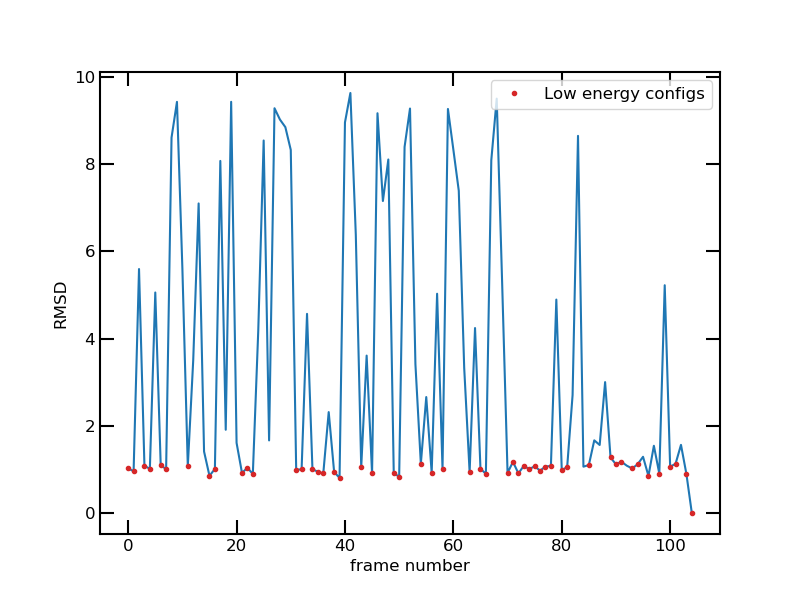
\includegraphics[width=\figwidth]{rmsd_cell1.png}
  \caption{RMSDs of cell 1 with respect to last frame.}
  \label{fig:rmsd_cell1}
\end{figure}

% subsection cell_1 (end)

\subsection{Cell 5} % (fold)
\label{sub:cell_5}

Figure~\ref{fig:potential_energy_cell5} shows the potential energies of all frames in the simulation of cell 5. As can be seen, after the zeroth frame, which has the typical higher energy of the tuning in phase, the potential energy somewhat stabilises around a value of \(\num{9.805(43)e6}\) for frames 1 through 38. But then for frame 39 and the following ones until the end of the simulation, the energy drops down to \(\num{8.220(8)e6}\). As seen in Figure~\ref{fig:potential_energy_cell5}, this is a reduction in both the potential energy itself as well as the deviation in potential energy from \(0.5 \%\) down to \(0.1 \%\), signifying that the second configuration is both energetically more favourable as well as more stable. The fact that this configuration was held for 38 frame though means that the existance of semi-stable configurations that are not the ground state are possible. To examine this effect further, cell 5 was simulated 2 more times. The resulting potential energies, together with the potential energies of the first simulation, can be seen in Figure~\ref{fig:potential_energy_cell5_all}. Clearly the second and third simulation run show the regular pattern that most other cells exhibit: the first one or two frames have a higher potential energy, and then it drops into a stable ground state where it remains. In particular the very similar potential energies of the ground state in all three simulations suggests that these ground states are in fact the same across all simulations. A analysis of the RMSDs between each frame to the last frame of the first simulation can be seen in Figure~\ref{fig:rmsd_cell5_all} and clearly shows that the ground states of all three simulations are in fact the same one.

\begin{figure}[ht]
\centering
  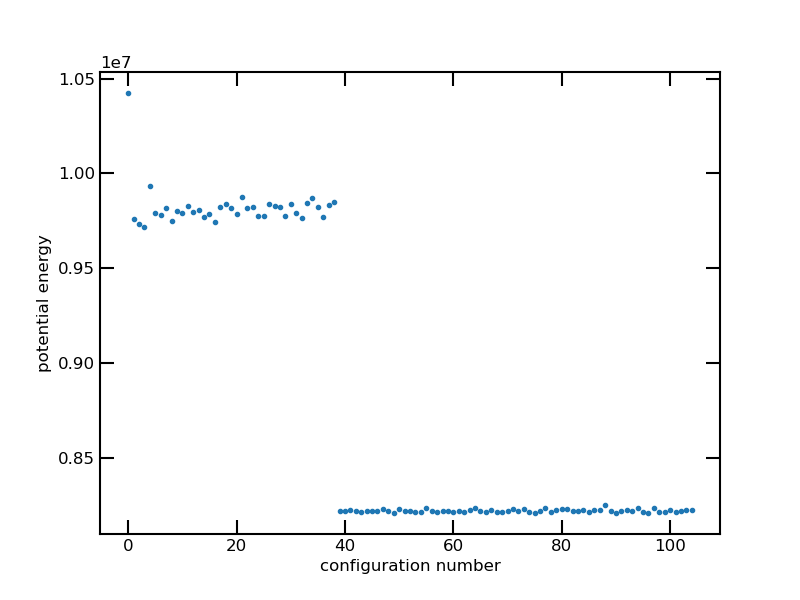
\includegraphics[width=\figwidth]{potential_energy_cell5.png}
  \caption{Potential energies of all frames in the simulation of cell 5.}
  \label{fig:potential_energy_cell5}
\end{figure}

\begin{figure}[ht]
\centering
  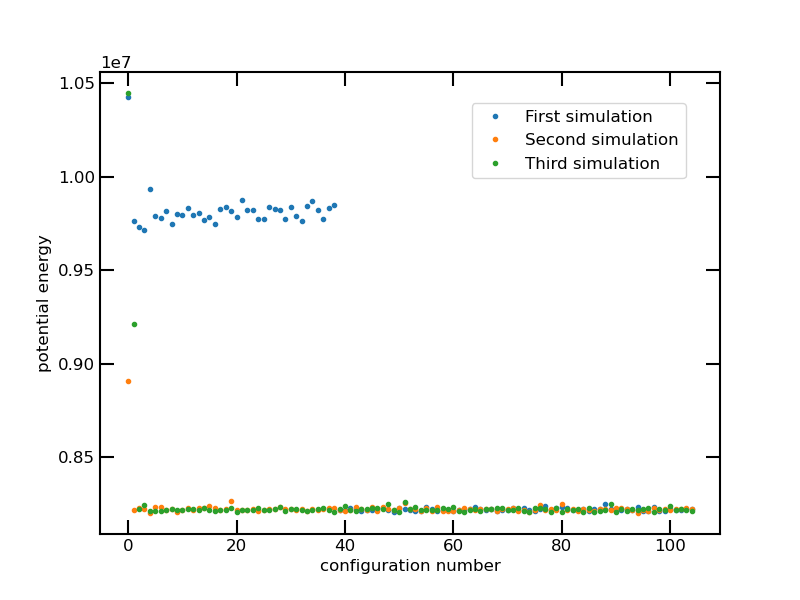
\includegraphics[width=\figwidth]{potential_energy_cell5_all.png}
  \caption{Potential energies of all frames in all three simulations of cell 5.}
  \label{fig:potential_energy_cell5_all}
\end{figure}

\begin{figure}[ht]
\centering
  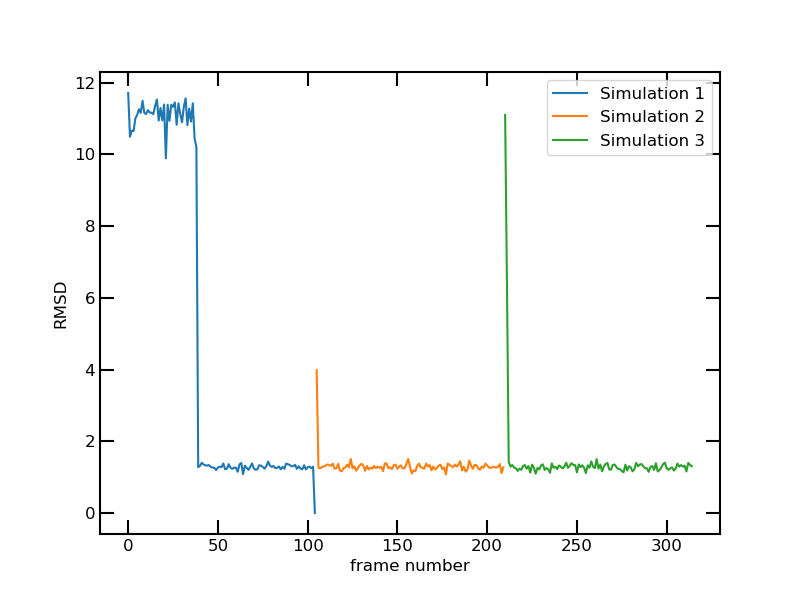
\includegraphics[width=\figwidth]{rmsd_cell5_all.png}
  \caption{RMSD of all three simulations of cell 5.}
  \label{fig:rmsd_cell5_all}
\end{figure}

% subsection cell_5 (end)

% section problems_with_the_simulation (end)


% chapter simulation (end)